%%%%%%%%%%%%%%%%%%%%%%%%%%%%%%%%%%%%%%%%%%%%%%%%%%%%%%%%%%%%%%%
%% Template from http://cameron.bracken.bz/beamer-template
%% Lecture slides for PHYS3550 General Relativity
%% Author: John Webb, School of Physics, UNSW. Started 1/12/12
%%%%%%%%%%%%%%%%%%%%%%%%%%%%%%%%%%%%%%%%%%%%%%%%%%%%%%%%%%%%%%%
%\documentclass[aspectratio=169,xcolor=x11names,compress]{beamer}
\documentclass[xcolor=x11names,compress]{beamer}

% General
%%%%%%%%%%%%%%%%%%%%%%%%%%%%%%%%%%%%%%%%%%%%%%%%%%%%%
\usepackage{tikz}
\usepackage[tikz]{bclogo}
%\usetikzlibrary{arrows,calc,plotmarks}
%\usepackage[latin1]{inputenc}
%\usepackage{graphicx}
%\usetikzlibrary{plotmarks}
%\usepackage{gnuplot-lua-tikz}
%\usepackage{mathpazo}%\usepackage{tikz}
%\usetikzlibrary{decorations.fractals}
%\usetikzlibrary{arrows,shapes}
%\usepackage{xifthen}
%%%%%%%%%%%%%%%%%%%%%%%%%%%%%%%%%%%%%%%%%%%%%%%%%%%%%%

%% Beamer Layout
%%%%%%%%%%%%%%%%%%%%%%%%%%%%%%%%%%%%%%%%%%%%%%%%%%%%%
\useoutertheme[subsection=false,shadow]{miniframes}
\useinnertheme{default}
%\usefonttheme{serif}
\usefonttheme{structurebold}
\usepackage{palatino}
\setbeamerfont{title like}{shape=\scshape}
\setbeamerfont{frametitle}{shape=\scshape}
\setbeamercolor*{lower separation line head}{bg=DeepSkyBlue4} 
\setbeamercolor*{normal text}{fg=black,bg=white} 
\setbeamercolor*{alerted text}{fg=red} 
\setbeamercolor*{example text}{fg=black} 
\setbeamercolor*{structure}{fg=black} 
\setbeamercolor*{palette tertiary}{fg=black,bg=black!10} 
\setbeamercolor*{palette quaternary}{fg=black,bg=black!10} 
\renewcommand{\(}{\begin{columns}}
\renewcommand{\)}{\end{columns}}
\newcommand{\<}[1]{\begin{column}{#1}}
\renewcommand{\>}{\end{column}}
%%JKW additions
%%%%%%%%%%%%%%%%%%%%%%%%%%%%%%%%%%%%%%%%%%%%%%%%%%%%%
\newcommand{\overbar}[1]{\mkern 1.5mu\overline{\mkern-1.5mu#1\mkern-1.5mu}\mkern 1.5mu}
%\newcommand{\doverbar}[1]{\mkern 1.5mu\overline{\mkern-1.5mu#1\mkern-1.5mu}\mkern 1.5mu}
\newcommand{\oframe}{\mathbb{O}}
\newcommand{\obarframe}{\overbar{\mathbb{O}}}
%\newcommand{\dobarframe}{\doverbar{\mathbb{O}}}
\newcommand{\dobarframe}{\overline{\overline{\mathbb{O}}}}

%%%%%%%%%%%%%%%%%%%%%%%%%%%%%%%%%%%%%%%%%%%%%%%%%%%%%
\begin{document}

%%%%%%%%%%%%%%%%%%%%%%%%%%%%%%%%%%%%%%%%%%%%%%%%%%%%%%
\begin{frame}
\title{PHYS3550 General Relativity}
%\subtitle{SUBTITLE}
\author{John Webb, University of New South Wales}
\date{
\begin{bclogo}[couleur = blue!30, arrondi = 0.1,barre=none,logo=, 
ombre = true, epOmbre = 0.25, couleurOmbre = black!30]{} 
{\hspace{1.3cm}\huge $G_{\mu \nu} = 8\pi G T_{\mu \nu} - \Lambda g_{\mu \nu}$
\vspace{0.5cm}}
\end{bclogo}
%\begin{bclogo}
%\begin{centering}{\Huge
%$G_{\mu \nu} = 8\pi G T_{\mu \nu} - \Lambda g_{\mu \nu}$
%}
%\end{centering}
%\end{shadowblock}
%\framebox{\includegraphics[width=2in]{AE_office_dayofdeath.jpg}}
%\begin{tikzpicture}[decoration=Koch curve type 2]
%\draw[DeepSkyBlue4] decorate{ decorate{ decorate{ (0,0) -- (3,0) }}}; 
%\end{tikzpicture}\\
%\vspace{1cm}
%\today
}
\titlepage
\end{frame}
%%%%%%%%%%%%%%%%%%%%%%%%%%%%%%%%%%%%%%%%%%%%%%%%%%%%%%

%%%%%%%%%%%%%%%%%%%%%%%%%%%%%%%%%%%%%%%%%%%%%%%%%%%%%%
\section{\scshape Preliminaries}
\begin{frame}{Contents}
\tableofcontents
\end{frame}
%%%%%%%%%%%%%%%%%%%%%%%%%%%%%%%%%%%%%%%%%%%%%%%%%%%%%%

%%%%%%%%%%%%%%%%%%%%%%%%%%%%%%%%%%%%%%%%%%%%%%%%%%%%%%
\subsection{Einstein's field equations}
\begin{frame}{Preliminaries}
\frametitle{What are Einstein's field equations?}
\begin{itemize}
\item General relativity is a theory of gravity.
\item Einstein's equations give a {\it geometric} description.
\item Classical view: motion of any object from A to B is 
due to a gradient in the gravitational field.
\item Einstein's ``new'' view: geometry of space (and time) 
changes continuously from A to B, so an object tends to ``fall''.
\end{itemize}
\end{frame}
%%%%%%%%%%%%%%%%%%%%%%%%%%%%%%%%%%%%%%%%%%%%%%%%%%%%%%

%%%%%%%%%%%%%%%%%%%%%%%%%%%%%%%%%%%%%%%%%%%%%%%%%%%%%%
\subsection{Out with the old}
\begin{frame}{Preliminaries}
\frametitle{Why abandon Newtonian concepts 1?}
\begin{itemize}
\item Many lines of thought motivated AE, not one single thought or observation.
\item Einstein from his famous 1905 paper: {\it It is known that Maxwell's 
electrodynamics, when applied to moving bodies, leads to asymmetries which do not
appear to be inherent in the phenomena}.  What he meant was that although
the experimental outcomes were consistent, the interpretations were not:
\item According to Maxwell's equations, when conductor stationary/magnet moving:
the changing magnetic field induces a current in the conductor, 
i.e. $\partial \vec{B}/\partial t \neq 0$, and $\nabla \times \vec{E} = 
- \partial \vec(B)/\partial t$.
\end{itemize}
\end{frame}

\begin{frame}{Preliminaries}
\frametitle{Why abandon Newtonian concepts 2?}
\begin{itemize}
\item BUT, when magnet stationary/conductor moving, $\vec{B} =  const \rightarrow
\partial \vec{B}/\partial t = 0 \rightarrow \vec{E} = 0$. Nevertheless, there's
still an emf, but now attributed to Lorentz force on the free electrons in
the conductor, $\vec{F} = q \left( \vec{E} + \vec{v} \times \vec{B} \right) 
= q \vec{v} \times \vec{B}$.  Thus the force doesn't come from an E-field
and 2 fundamentally different interpretations are needed for the same phenomenon.  
{\color{red} {\bf FAIL!}}
\item Newton's 3 laws are all invariant in inertial reference frames.
Thus {\it mechanical} laws seem absolute (Newton mechanical relativity
principle). Why not extend this to apply to {\it all} physical laws?
\end{itemize}
\end{frame}

\begin{frame}{Preliminaries}
\frametitle{Why abandon Newtonian concepts 3?}
\begin{itemize}
\item SR was completed in 1905.  $c$ was declared an absolute constant --
inevitable conclusion that Galilean velocity addition was wrong;
kinematics needed a more consistent description.
\item SR showed that co-ordinate measurements depended on the reference
frame of the observer, which appeared to conflict with the generally
accepted view that physical laws should be absolute and also `unified''.
\item Null-result from Michelson--Morley experiment.  There was no 
``aether'' and no ``absolute reference frame''.
\item There was thus no ``absolute space'', contrary to Newton's claim.
\end{itemize}
\end{frame}
%%%%%%%%%%%%%%%%%%%%%%%%%%%%%%%%%%%%%%%%%%%%%%%%%%%%%%

%%%%%%%%%%%%%%%%%%%%%%%%%%%%%%%%%%%%%%%%%%%%%%%%%%%%%%
\begin{frame}{Homework}
\begin{columns}
\column{\textwidth}
\setbeamercolor{uppercol}{fg=white,bg=red!54!black}
\setbeamercolor{lowercol}{fg=black,bg=red!10}
\begin{beamerboxesrounded}[upper=uppercol,lower=lowercol,shadow=true]{Homework 1}
A comprehensive discussion of what motivated Einstein's special
theory is given in the excellent book:\\
{\it Relativity - Special, General and Cosmological},\\
Wolfgang Rindler, 2nd edition, 2006, Oxford University Press.\\

Read chapter 1, from the start up to and including Section 1.11.\\

(The book is online -- Google ``Rindler relativity pdf'').
\end{beamerboxesrounded}
\end{columns}
\end{frame}
%%%%%%%%%%%%%%%%%%%%%%%%%%%%%%%%%%%%%%%%%%%%%%%%%%%%%%

%%%%%%%%%%%%%%%%%%%%%%%%%%%%%%%%%%%%%%%%%%%%%%%%%%%%%%
\section{\scshape Special Relativity}
\subsection{The 2 postulates of Special Relativity}
\begin{frame}{Special Relativity}
\frametitle{Postulates of Special Relativity}

\setbeamercolor{uppercol}{fg=white,bg=green!40!black}
\setbeamercolor{lowercol}{fg=black,bg=green!10}
\begin{beamerboxesrounded}[upper=uppercol,lower=lowercol,shadow=true]
{1. The Relativity Principle}
All intertial reference frames are equivalent for the performance 
of all physical experiments ie. the laws of physics are identical 
in all intertial reference frames.
\end{beamerboxesrounded}

\bigskip

\setbeamercolor{uppercol}{fg=white,bg=blue!40!black}
\setbeamercolor{lowercol}{fg=black,bg=blue!10}
\begin{beamerboxesrounded}[upper=uppercol,lower=lowercol,shadow=true]
{2. Invariance of the speed of light}
In empty space, light travels rectilinearly (i.e. in straight lines) 
at fixed speed c, in every direction in every inertial reference frame,
independent of the state of motion of the emitting body and independent 
of the state of motion of the observer.
\end{beamerboxesrounded}

\end{frame}
%%%%%%%%%%%%%%%%%%%%%%%%%%%%%%%%%%%%%%%%%%%%%%%%%%%%%%

%%%%%%%%%%%%%%%%%%%%%%%%%%%%%%%%%%%%%%%%%%%%%%%%%%%%%%
\subsection{Natural units}
\begin{frame}{Natural units}
The meter and second are arbitrary units introduced for convenience.  
It's simpler to use a more ``natural'' system, so that a suitable 
universal constant becomes a unit.  For GR, we use the speed 
of light, $c$, as a natural unit of speed.\\
\bigskip
Since speed = distance/time, we therefore need to have distance and
time measured in the same units, to have $c$ dimensionless.\\
\bigskip
If this sounds strange, recall we often measure distance 
in ``light years'', i.e. the distance light travels in 1 year.\\
\bigskip
So $c = $(distance light travels per unit time)/(unit time)
and since the top is now measured in $m$, we must have time measured in
$m$ as well, so $c = 1$.
\end{frame}
%%%%%%%%%%%%%%%%%%%%%%%%%%%%%%%%%%%%%%%%%%%%%%%%%%%%%%

%%%%%%%%%%%%%%%%%%%%%%%%%%%%%%%%%%%%%%%%%%%%%%%%%%%%%%
\subsection{Co-ordinates}
\begin{frame}{Special Relativity}
\frametitle{Co-ordinates notation}
\begin{itemize}
%\item Conventional notation $\mathbf{x}$ $(=t,x,y,x)$ (i.e. $t$ first).
\item Conventional notation $(t,x,y,x)$, i.e. $t$ first.
\item Event -- a single fixed point
in a continuous space.
\item World line -- $x$ as f($t$) for a particle.  
\item Slope of world line $dt/dx = 1/v$.
\item Photons have $45^{\circ}$ world lines --  {\em always}.
\item Alternative representation.  Instead of $(t,x,y,x)$, use
$x^0, x^1, x^2, x^3)$, where $\alpha$ is any Greek 
index e.g. $\alpha, \beta, \gamma, \mu, \nu$.
\item Spatial co-ordinates only can be indicated using Latin indices
e.g. $x^a, x^b, x^i, x^j$ etc.  If no value of the index given, $x^i$ can
be any of the 3 spatial coordinates.
\end{itemize}
\end{frame}
%%%%%%%%%%%%%%%%%%%%%%%%%%%%%%%%%%%%%%%%%%%%%%%%%%%%%%

%%%%%%%%%%%%%%%%%%%%%%%%%%%%%%%%%%%%%%%%%%%%%%%%%%%%%%
\subsection{Spacetime (Minkowski) diagrams}
\begin{frame}{Special Relativity}
\frametitle{Spacetime (or Minkowski) diagrams}

\begin{center} 
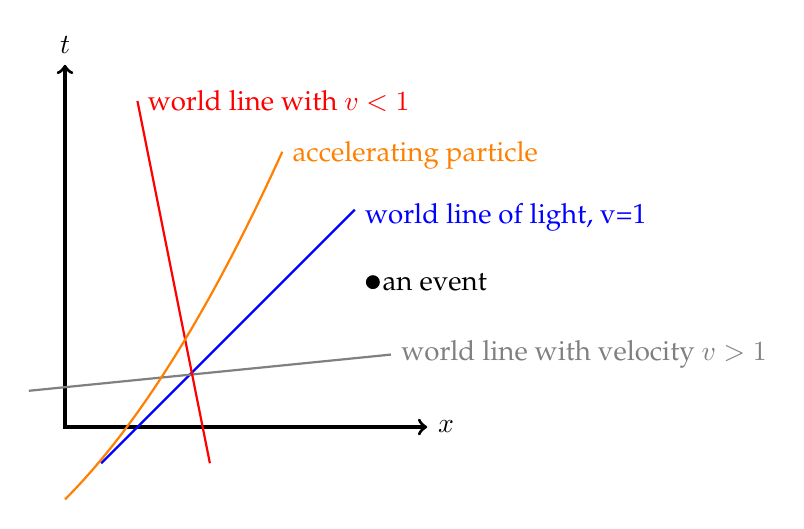
\begin{tikzpicture}[scale=4.6]
\draw [<->,very thick] (0,1) node [above] {$t$} -- (0,0) -- (1,0) 
   node [right] {$x$};
\draw [thick,blue] (0.1,-0.1) -- (0.8,0.6) node [right] at 
   (0.8,0.58) {world line of light, v=1};
\draw [thick,gray] (-.1,0.1) -- (0.9,0.2) node [right]
   {world line with velocity $v > 1$};
\draw [thick,red] (0.4,-.1) -- (0.2,0.9) node [right]
   {world line with $v < 1$};
\draw [thick,orange,domain=0:0.6] plot (\x, {-0.2+\x+\x*\x})
   node [right] at (0.6,0.75) {accelerating particle};
\filldraw [black] (0.85,0.4) circle (0.5pt) node [right] {an event};
\end{tikzpicture}
\end{center}

\end{frame}
%%%%%%%%%%%%%%%%%%%%%%%%%%%%%%%%%%%%%%%%%%%%%%%%%%%%%%

%%%%%%%%%%%%%%%%%%%%%%%%%%%%%%%%%%%%%%%%%%%%%%%%%%%%%%
\begin{frame}
\frametitle{Hermann Minkowski 1864--1909}
\begin{columns}[c] 
\column{3.0in}
b.Poland, d.Germany. Institutions: G\"ottingen, ETH Zurich. Einstein's
teacher.  1907 described SR geometrically -- this influenced Einstein's GR
development.  Died aged 44 appendicitis.  Famous 1908 quote:
\vspace{0.2in}\newline
\color{blue}{
{\it "The views of space and time which I wish to lay before you have sprung
from the soil of experimental physics, and therein lies their strength. They
are radical. Henceforth space by itself, and time by itself, are doomed to
fade away into mere shadows, and only a kind of union of the two will preserve
an independent reality."}
}
\column{1.5in} 
%\framebox{\includegraphics[width=1.5in]{images/De_Raum_zeit_Minkowski_Bild.jpg}} 
\end{columns}
\end{frame}
%%%%%%%%%%%%%%%%%%%%%%%%%%%%%%%%%%%%%%%%%%%%%%%%%%%%%%

%%%%%%%%%%%%%%%%%%%%%%%%%%%%%%%%%%%%%%%%%%%%%%%%%%%%%%
\subsection{Inertial observers and some assumptions}
\begin{frame}
\frametitle{Inertial observers and some assumptions}
SR deals only with non-accelerating (inertial) observers.\\
\bigskip
SR assumes all clocks can be synchronised, and that they
run at the same rate in their rest frames.\\
\bigskip
SR applies only to a spacetime with Euclidean geometry.\\
\bigskip
Note the presence of a gravitational field violates all the above,
so we make the approximation that any field is weak. 
\end{frame}
%%%%%%%%%%%%%%%%%%%%%%%%%%%%%%%%%%%%%%%%%%%%%%%%%%%%%%

%%%%%%%%%%%%%%%%%%%%%%%%%%%%%%%%%%%%%%%%%%%%%%%%%%%%%%
\begin{frame}
\frametitle{Illustrating 2 inertial observers on the same spacetime diagram 1}
Assume 2 observers $\oframe$ and $\obarframe$.  Assume $\obarframe$ moves with
velocity $v$ along $x$ direction relative to $\oframe$ (i.e. assume axes
are aligned -- makes things easier, no loss of generality).\\
$\bar{t}$ is simply  $\obarframe$'s world line, (or, by definition,
the locus of events occurring at $\bar{x}=0$).
\begin{center}
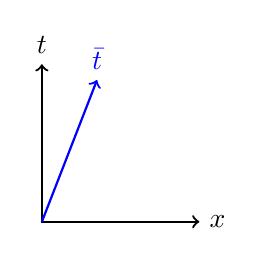
\begin{tikzpicture}[scale=2]
\draw [<->,thick] (0,1) node [above] {$t$} -- (0,0) -- (1,0) 
   node [right] {$x$};
\draw [->,thick,blue] (0,0) -- (0.35,0.9) node [above] {$\bar{t}$};
\end{tikzpicture}
\end{center}
The $\bar{x}=0$ axis is thus, also by definition, the locus of events
occurring at $\bar{t}=0.$
\end{frame}
%%%%%%%%%%%%%%%%%%%%%%%%%%%%%%%%%%%%%%%%%%%%%%%%%%%%%%

%%%%%%%%%%%%%%%%%%%%%%%%%%%%%%%%%%%%%%%%%%%%%%%%%%%%%%
\begin{frame}
\frametitle{Illustrating 2 inertial observers on the same spacetime diagram 2}

\begin{columns}
\column{0.5\textwidth}
Consider the following 1-dimensional thought experiment in $\obarframe$'s 
rest-frame.  A light ray is emitted from the origin, travels along x,
encounters a mirror a distance $a$ away, then is reflected back to the 
origin.  The spacetime representation is this:

\column{0.5\textwidth}
%\begin{center}
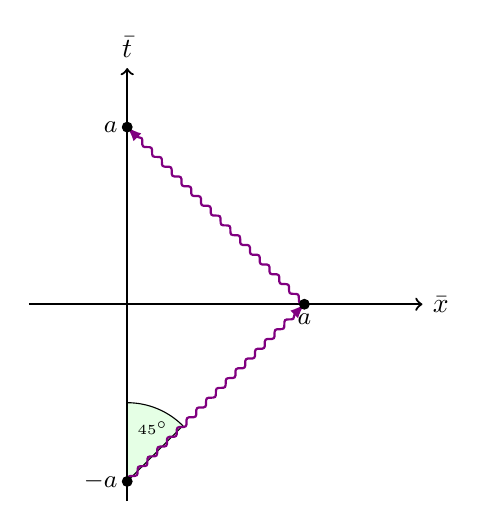
\begin{tikzpicture}[scale=2.5]
%AXES
\draw [<->,thick] (0,1.2) node [above] {$\bar{t}$} -- (0,0) -- (1.5,0) 
   node [right] {$\bar{x}$};
\draw [-,thick] (-0.5,0) -- (0,0);
\draw [-,thick] (0,-1) -- (0,0); 
%ANGLE
\filldraw [fill=green!10] (0,-0.9) -- (0,-0.5) arc (90:45:0.4) -- cycle;
\node at (0.13,-0.63) {\tiny{$45^{\circ}$}};
%LIGHT RAYS
\draw [-latex,thick, color=red!50!blue,decorate,decoration={snake,amplitude=.3mm, 
   segment length=5pt,post length=1mm}] (0,-0.9) -- (0.9,0);
\draw [-latex,thick, color=red!50!blue,decorate,decoration={snake,amplitude=.3mm, 
   segment length=5pt,post length=1mm}] (0.9,0) -- (0,0.9);
\filldraw [black] (0,0.9) circle (0.7pt) node [left] {\small{$a$}};
\filldraw [black] (0.9,0) circle (0.7pt) node [below] {\small{$a$}};
\filldraw [black] (0,-0.9) circle (0.7pt) node [left] {\small{$-a$}};
\end{tikzpicture}
%\end{center}

\end{columns}

\end{frame}
%%%%%%%%%%%%%%%%%%%%%%%%%%%%%%%%%%%%%%%%%%%%%%%%%%%%%%

%%%%%%%%%%%%%%%%%%%%%%%%%%%%%%%%%%%%%%%%%%%%%%%%%%%%%%
\begin{frame}
\frametitle{Illustrating 2 inertial observers on the same spacetime diagram 3}
\begin{columns}

\column{0.5\textwidth}
In the previous diagram, since the mirror is distance $a$ along
$\bar{x}$, and since light rays must lie at $45^{\circ}$, the time
interval between emission and arrival must be $2a$.\\
\bigskip
Consider this in $\oframe$'s rest-frame.  2nd postulate means light
rays are still at $45^{\circ}$.  Incident and reflected rays must
intersect at mirror, on the $\bar{x}$ axis.

\column{0.5\textwidth}
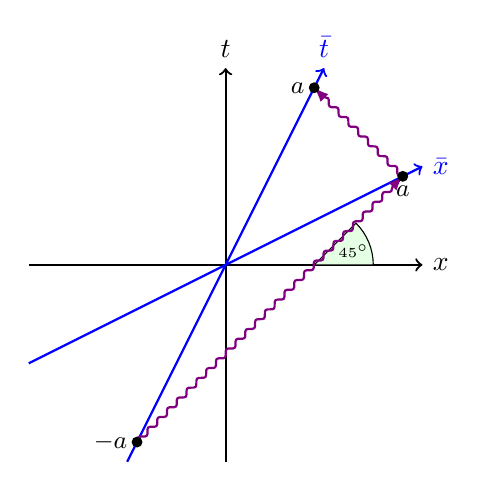
\begin{tikzpicture}[scale=2.5]
%O's AXES
\draw [->,thick] (0,-1) -- (0,0) -- (0,1) node [above] {$t$};
\draw [->,thick] (-1,0) -- (0,0) -- (1,0) node [right] {$x$};
%O bar's axes
\draw [->,thick,blue] (-0.5,-1) -- (0,0) -- (0.5,1) node [above] {$\bar{t}$};
\draw [->,thick,blue] (-1,-0.5) -- (0,0) -- (1,0.5) node [right] {$\bar{x}$};
%ANGLE
\filldraw [fill=green!10] (0.45,0) -- (0.75,0) arc (0:45:0.3) -- cycle;
\node at (0.65,0.07) {\tiny{$45^{\circ}$}};
%LIGHT RAYS
\draw [-latex,thick, color=red!50!blue,decorate,decoration={snake,amplitude=.3mm, 
   segment length=5pt,post length=1mm}] (-0.45,-0.9) -- (0.9,0.45);
\draw [-latex,thick, color=red!50!blue,decorate,decoration={snake,amplitude=.3mm, 
   segment length=5pt,post length=1mm}] (0.9,0.45) -- (0.45,0.9);
%EVENTS
\filldraw [black] (-0.45,-0.9) circle (0.7pt) node [left] {\small{$-a$}};
\filldraw [black] (0.9,0.45) circle (0.7pt) node [below] {\small{$a$}};
\filldraw [black] (0.45,0.9) circle (0.7pt) node [left] {\small{$a$}};
\end{tikzpicture}

\end{columns}
\end{frame}
%%%%%%%%%%%%%%%%%%%%%%%%%%%%%%%%%%%%%%%%%%%%%%%%%%%%%%

%%%%%%%%%%%%%%%%%%%%%%%%%%%%%%%%%%%%%%%%%%%%%%%%%%%%%%
\begin{frame}
\frametitle{Simultaneity is observer--dependent}

\begin{columns}
\column{0.5\textwidth}
Now consider lines A and B:  
\begin{itemize}
\item Only events falling along A 
will be regarded by $\oframe$ as simultaneous. 
\item Only events falling along B 
will be regarded by $\obarframe$ as simultaneous.
\end{itemize}
\bigskip
\setbeamercolor{uppercol}{fg=white,bg=blue!40!black}
\setbeamercolor{lowercol}{fg=white,bg=red!40!black}
\begin{beamerboxesrounded}[upper=uppercol,lower=lowercol,shadow=true]
{Fundamental consequence of the constancy of $c$:}
{Different inertial observers do not agree on simultaneity!}
\end{beamerboxesrounded}

\column{0.5\textwidth}
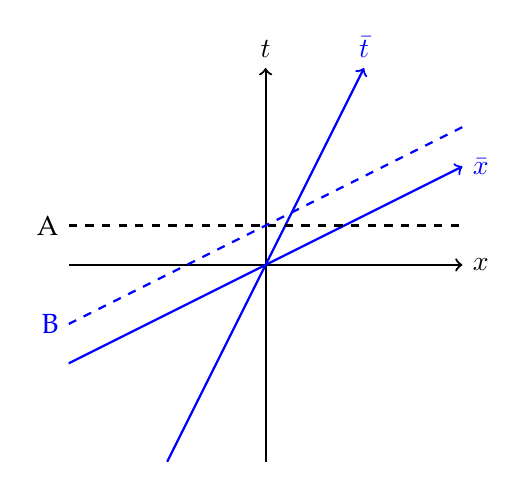
\begin{tikzpicture}[scale=2.5]
%O'S AXES
\draw [->,thick] (0,-1) -- (0,0) -- (0,1) node [above] {$t$};
\draw [->,thick] (-1,0) -- (0,0) -- (1,0) node [right] {$x$};
%O BAR'S AXES
\draw [->,thick,blue] (-0.5,-1) -- (0,0) -- (0.5,1) node [above] {$\bar{t}$};
\draw [->,thick,blue] (-1,-0.5) -- (0,0) -- (1,0.5) node [right] {$\bar{x}$};
%LINE OF SIMULTANEITY FOR O
\draw [-,thick,dashed] (-1,0.2) node [left] {A} -- (0,0.2) -- (1,0.2);
%LINE OF SIMULTANEITY FOR O BAR
\draw [-,blue,thick,dashed] (-1,-0.3) node [left] {B} -- (0,0.2) -- (1,0.7);
\end{tikzpicture}

\end{columns}
\end{frame}
%%%%%%%%%%%%%%%%%%%%%%%%%%%%%%%%%%%%%%%%%%%%%%%%%%%%%%

%%%%%%%%%%%%%%%%%%%%%%%%%%%%%%%%%%%%%%%%%%%%%%%%%%%%%%
\begin{frame}
\frametitle{The interval}

\begin{columns}
\column{0.6\textwidth}
Consider the previous photon emission (E) and reflection (R) events:
Let the co-ordinate differences measured by $\oframe$ 
be $\Delta t$ and $\Delta x$.
Light rays are $45^{\circ}$, so
$-(\Delta t)^2 + (\Delta x)^2 = 0$.

\column{0.4\textwidth}
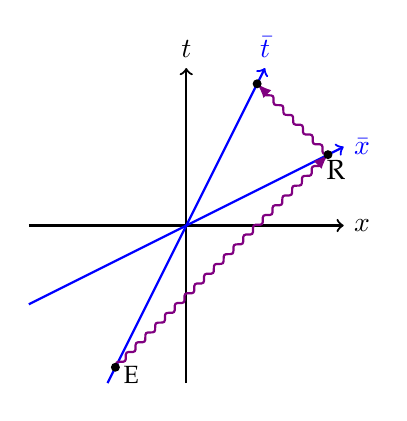
\begin{tikzpicture}[scale=2]
% O's AXES
\draw [->,thick] (0,-1) -- (0,0) -- (0,1) node [above] {$t$};
\draw [->,thick] (-1,0) -- (0,0) -- (1,0) node [right] {$x$};
% OBAR'S axes
\draw [->,thick,blue] (-0.5,-1) -- (0,0) -- (0.5,1) node [above] {$\bar{t}$};
\draw [->,thick,blue] (-1,-0.5) -- (0,0) -- (1,0.5) node [right] {$\bar{x}$};
% LIGHT RAYS
\draw [-latex,thick, color=red!50!blue,decorate,decoration={snake,amplitude=.3mm, 
   segment length=5pt,post length=1mm}] (-0.45,-0.9) -- (0.9,0.45);
\draw [-latex,thick, color=red!50!blue,decorate,decoration={snake,amplitude=.3mm, 
   segment length=5pt,post length=1mm}] (0.9,0.45) -- (0.45,0.9);
% EVENTS
\filldraw [black] (-0.45,-0.9) circle (0.7pt);
\node at (-0.35,-0.95) {\small{E}};
\filldraw [black] (0.9,0.45) circle (0.7pt); 
\node at (0.95,0.35) {R};
\filldraw [black] (0.45,0.9) circle (0.7pt);

\end{tikzpicture}

\end{columns}

In 4 dimensions, for a light ray specifically,
$-(\Delta t)^2 + (\Delta x)^2 + (\Delta y)^2 + (\Delta z)^2 = 0$\\
\bigskip

%\setbeamercolor{uppercol}{fg=white,bg=blue!40!black}
\setbeamercolor{lowercol}{fg=white,bg=red!40!black}
\begin{beamerboxesrounded}[upper=uppercol,lower=lowercol,shadow=true]
{}
{More generally, for any 2 events not on a light world line,\\
$-(\Delta t)^2 + (\Delta x)^2 + (\Delta y)^2 + (\Delta z)^2 = (\Delta s)^2$\\
$(\Delta s)^2$ is called {\color{red} {\it the squared interval}}}.
\end{beamerboxesrounded}

\end{frame}
%%%%%%%%%%%%%%%%%%%%%%%%%%%%%%%%%%%%%%%%%%%%%%%%%%%%%%

%%%%%%%%%%%%%%%%%%%%%%%%%%%%%%%%%%%%%%%%%%%%%%%%%%%%%%
\begin{frame}
\frametitle{Interval invariance from first principles 1}

We already saw that, for photons in $\oframe$,\\
$-(\Delta t)^2 + (\Delta x)^2 + (\Delta y)^2 + (\Delta z)^2 = 0$\\
The constancy of $c$ thus also requires\\
$-(\Delta \bar{t})^2 + (\Delta \bar{x})^2 + (\Delta \bar{y})^2 
+ (\Delta \bar{z})^2 = 0$
\bigskip

\setbeamercolor{lowercol}{fg=white,bg=blue!40!black}
\begin{beamerboxesrounded}[upper=uppercol,lower=lowercol,shadow=true]
{}{We will now prove that $(\Delta \bar{s})^2 = (\Delta s)^2$}
\end{beamerboxesrounded}
\bigskip
Consider 2 dimensions initially (simpler).  Since frames are inertial,
assume that $\bar x, \bar y$ are linear combinations
of $x, y$, i.e.\\
$\bar{x} = a_1x + a_2y$\\
$\bar{y} = b_1x + b_2y$\\
For convenience, take $\oframe$ and $\obarframe$ origins coincident at
$t = \bar{t} = 0$.
\end{frame}
%%%%%%%%%%%%%%%%%%%%%%%%%%%%%%%%%%%%%%%%%%%%%%%%%%%%%%

%%%%%%%%%%%%%%%%%%%%%%%%%%%%%%%%%%%%%%%%%%%%%%%%%%%%%%
\begin{frame}
\frametitle{Interval invariance from first principles 2}

The interval measured in $\oframe$ and $\obarframe$ is
%$\overline{\mathbb{O}}$ $\overbar{\mathbb{O}}$ is
\begin{align*}
\bar{s}^2 & = \bar{x}^2 + \bar{y}^2 \\
          & = a_1^2 x^2 + a_2^2 y^2 + 2 a_1 a_2 xy \\
          & + b_1^2 x^2 + b_2^2 y^2 + 2 b_1 b_2 xy
\end{align*}
which can be written as the summation
\begin{align*}
\bar{s}^2 & = \sum\limits_{\alpha=1}^2 \sum\limits_{\beta=1}^2 
m_{\alpha\beta} x^{\alpha} x^{\beta}
\end{align*}
or, more generally, going to 4-dimensions and reverting to the previous
notation for co-ordinate differences,
\begin{align}
(\Delta \bar{s})^2 & = \sum\limits_{\alpha=0}^3 \sum\limits_{\beta=0}^3 m_{\alpha\beta}
(\Delta x^{\alpha})(\Delta x^{\beta}) \label{dssum}
\end{align}

\end{frame}
%%%%%%%%%%%%%%%%%%%%%%%%%%%%%%%%%%%%%%%%%%%%%%%%%%%%%%

%%%%%%%%%%%%%%%%%%%%%%%%%%%%%%%%%%%%%%%%%%%%%%%%%%%%%%
\begin{frame}
\frametitle{Interval invariance from first principles 3}

Now for photons, for which $(\Delta s)^2 = 0$,
\begin{align*}
(\Delta t)^2 & = (\Delta x)^2 + (\Delta y)^2 + (\Delta z)^2 = (\Delta r)^2 \text { say}
\end{align*}
Substituting this into equation (\ref{dssum}) gives
\begin{align*}
(\Delta \bar{s})^2 & = m_{00} (\Delta r)^2 + 2 \Delta r \sum\limits_{i=1}^3 m_{0i}
  \Delta x^i + \sum\limits_{i=1}^3 \sum\limits_{j=1}^3 m_{ij} \Delta x^i \Delta x^j
\end{align*}
However if $(\Delta s)^2 = 0$, then $(\Delta \bar{s})^2 = 0$ too, which results in
\begin{align*}
m_{0i} & = 0 & \text{ for } i=1,2,3 \\
m_{ij} & = -m_{00} \delta_{ij} & \text{ for } i=1,2,3
\end{align*}
where the Kroneker $\delta_{ij}$ is
\begin{align*}
\delta_{ij} & = 1 & \text{ if } i = j \\
            & = 0 & \text{ if } i \ne j
\end{align*}

\end{frame}
%%%%%%%%%%%%%%%%%%%%%%%%%%%%%%%%%%%%%%%%%%%%%%%%%%%%%%

%%%%%%%%%%%%%%%%%%%%%%%%%%%%%%%%%%%%%%%%%%%%%%%%%%%%%%
\begin{frame}
\frametitle{Interval invariance from first principles 4}

Equation (1) now simplifies to
\begin{align*}
(\Delta \bar{s})^2 & = -m_{00} \left[- (\Delta t)^2 + (\Delta x)^2 + (\Delta y)^2 
+ (\Delta z)^2 \right]
\end{align*}

However $m_{00}$ depends only on the relative velocity $\vec{\bf v}$ 
between $\oframe$ and $\obarframe$.  But the first postulate (Relativity 
Principle) requires that space is isotropic (no preferred direction),  
i.e. $m_{00} = -f(|v|)$, so
\setbeamercolor{lowercol}{fg=white,bg=red!40!black}
\begin{beamerboxesrounded}[upper=uppercol,lower=lowercol,shadow=true]
{}{\begin{align}
(\Delta \bar{s})^2 & = f(|v|) (\Delta s)^2 \label{fv}
\end{align}}
\end{beamerboxesrounded}

(Note one could {\it assume} equation (\ref{fv}).  All we have done so far is to 
show (\ref{fv}) follows from the assumption of linear coordinate transformations).

\end{frame}
%%%%%%%%%%%%%%%%%%%%%%%%%%%%%%%%%%%%%%%%%%%%%%%%%%%%%%

%%%%%%%%%%%%%%%%%%%%%%%%%%%%%%%%%%%%%%%%%%%%%%%%%%%%%%
\begin{frame}
\frametitle{Interval invariance from first principles 5. What is $f(|v|)$?}

\begin{columns}
\column{0.45\textwidth}
Consider a rod, stationary in $\oframe$, lying along the $y$ axis.
(Yes, the $y$ axis, not $x$).
Events A and B are the ends of the rod at $t=0$.\\
\bigskip
\setbeamercolor{lowercol}{fg=black,bg=yellow}
\begin{beamerboxesrounded}[upper=uppercol,lower=lowercol,shadow=true]
{}{$\oframe$ sees events A and B \\ simultaneously.}
\end{beamerboxesrounded}
\bigskip
Let $\obarframe$ move with speed 
$v$ in the positive $x$ direction relative to $\oframe$. \\
\bigskip
How does $\obarframe$ see A and B?

\column{0.55\textwidth}

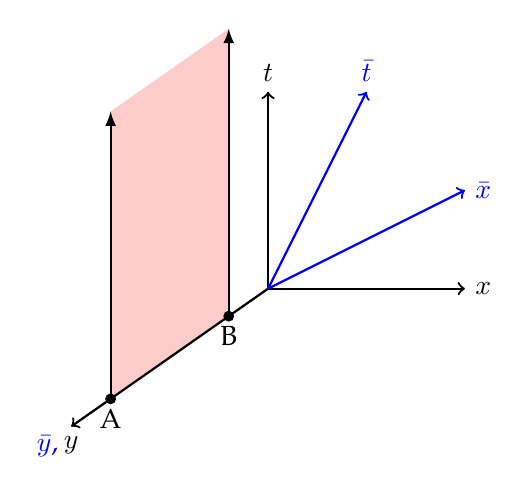
\begin{tikzpicture}[scale=2.5]
% FILL BETWEEN ROD WORLD LINES
\path [fill=red,red!20!white] (-0.8,-0.56) -- (-0.2,-0.14) -- (-0.2,1.32)-- (-0.8,0.9);
% O'S AXES
\draw [->,thick] (0,0) -- (0,1) node [above] {$t$};
\draw [->,thick] (0,0) -- (1,0) node [right] {$x$};
\draw [->,thick] (0,0) -- (-1,-0.7) node[below] {$y$};
% OBAR'S axis
\draw [->,thick,blue] (0,0) -- (0.5,1) node [above] {$\bar{t}$};
\draw [->,thick,blue] (0,0) -- (1,0.5) node [right] {$\bar{x}$};
% WORLD LINES OF ROD ENDS
\draw [-latex,thick] (-0.8,-0.56) -- (-0.8,0.9);
\draw [-latex,thick] (-0.2,-0.14) -- (-0.2,1.32);
% EVENTS
\filldraw [black] (-0.8,-0.56) circle (0.7pt);
\node at (-0.8,-0.66) {A};
\filldraw [black] (-0.2,-0.14) circle (0.7pt);
\node at (-0.2,-0.24) {B};
% YBAR LABEL
\node at (-1.12,-0.8) {\color{blue} $\bar{y}$,};
\end{tikzpicture}

\end{columns}

\end{frame}
%%%%%%%%%%%%%%%%%%%%%%%%%%%%%%%%%%%%%%%%%%%%%%%%%%%%%%

%%%%%%%%%%%%%%%%%%%%%%%%%%%%%%%%%%%%%%%%%%%%%%%%%%%%%%
\begin{frame}
\frametitle{Interval invariance from first principles 6. What is $f(|v|)$?}

\begin{columns}
\column{0.55\textwidth}

Rotate the previous diagram so the $ty$ plane lies in the page.
The $x$ axis thus now points into the page.\\
\bigskip
The $\bar{t}$ axis has to lie in the $tx$ plane.  Thus the $\bar{t}$ axis
must be perpendicular to the $y$ axis.  
(If this seems odd, remember
there is no component of the velocity in the $y$ direction).\\
\bigskip

\setbeamercolor{lowercol}{fg=black,bg=yellow}
\begin{beamerboxesrounded}[upper=uppercol,lower=lowercol,shadow=true]
{}{Therefore, $\obarframe$ must
also see events \\ A and B simultaneously.}
\end{beamerboxesrounded}

\column{0.45\textwidth}

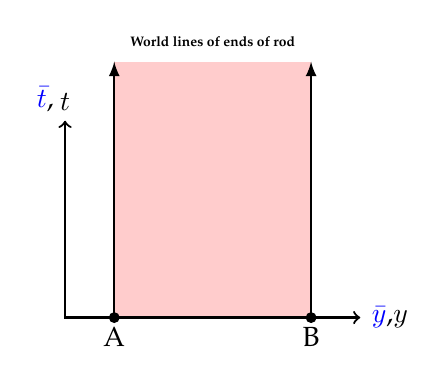
\begin{tikzpicture}[scale=2.5]
% FILL ROD WORLD LINES
\path [fill=red,red!20!white] (0.25,0) rectangle (1.25,1.3);
% AXES
\draw [<->,thick] (0,1) node [above] {$t$} -- (0,0) -- (1.5,0);
% WORLD LINES OF FRONT AND END OF ROD
\draw [-latex,thick] (0.25,0) -- (0.25,1.3);
\draw [-latex,thick] (1.25,0) -- (1.25,1.3);
\node at (0.75,1.4) {\tiny\bf World lines of ends of rod};
% EVENTS
\filldraw [black] (0.25,0) circle (0.7pt);
\node at (0.25,-0.1) {A};
\filldraw [black] (1.25,0) circle (0.7pt);
\node at (1.250,-0.1) {B};
% AXIS LABELS
\node at (-0.1,1.11) {{\color{blue} $\bar{t}$},};
\node at (1.65,0) {{\color{blue} $\bar{y}$},$y$};
\end{tikzpicture}

\end{columns}

\end{frame}
%%%%%%%%%%%%%%%%%%%%%%%%%%%%%%%%%%%%%%%%%%%%%%%%%%%%%%

%%%%%%%%%%%%%%%%%%%%%%%%%%%%%%%%%%%%%%%%%%%%%%%%%%%%%%
\begin{frame}
\frametitle{Interval invariance from first principles 7. What is $f(|v|)$?}

Since A and B lie on the $y$ axis, the squared interval between 
A and B measured by $\oframe$ equals the square of the length of 
the rod measured by $\oframe$.\\
\bigskip
Since the $y$ and $\bar{y}$ coincide, the same holds for $\obarframe$.\\
\bigskip
Thus, from equation (\ref{fv})\\
\bigskip
\setbeamercolor{lowercol}{fg=black,bg=yellow}
\begin{beamerboxesrounded}[upper=uppercol,lower=lowercol,shadow=true]
{}{(Length of rod in $\oframe$)$^2$ = $f(|v|)$ (Length of 
rod in $\obarframe$)$^2$}
\end{beamerboxesrounded}

\end{frame}
%%%%%%%%%%%%%%%%%%%%%%%%%%%%%%%%%%%%%%%%%%%%%%%%%%%%%%

%%%%%%%%%%%%%%%%%%%%%%%%%%%%%%%%%%%%%%%%%%%%%%%%%%%%%%
\begin{frame}
\frametitle{Interval invariance from first principles 8. What is $f(|v|)$?}

Now consider 3 frames, $\oframe$, $\obarframe$, and $\dobarframe$.\\
$\obarframe$ moves at +v along $x$ relative to $\oframe$.\\
$\dobarframe$ moves at --v along $x$ relative to $\obarframe$.\\
From equation (\ref{fv}),

\begin{equation*} \left.
\begin{aligned} 
(\Delta \bar{\bar{s}})^2 = f(|v|) (\Delta \bar{s})^2 \\
(\Delta \bar{s})^2 = f(|v|) (\Delta s)^2
\end{aligned} \right\}
\quad \Longrightarrow (\Delta \bar{\bar{s}})^2 = [f(|v|)]^2 (\Delta s)^2
\end{equation*}

However $\obarframe$ and $\dobarframe$ are identical, so 
$(\Delta \bar{\bar{s}})^2 = (\Delta s)^2$ i.e. $f(|v|)^2 = 1$,
and $f(|v|) = 1$ (not $-1$ since square of length of rod must
be positive).  Therefore, finally,
\setbeamercolor{lowercol}{fg=black,bg=yellow}
\setbeamercolor{uppercol}{fg=white,bg=blue}
\begin{beamerboxesrounded}[upper=uppercol,lower=lowercol,shadow=true]
{The interval is invariant!}{($\Delta \bar{s})^2 = (\Delta s)^2$}
\end{beamerboxesrounded}

\end{frame}
%%%%%%%%%%%%%%%%%%%%%%%%%%%%%%%%%%%%%%%%%%%%%%%%%%%%%%

%%%%%%%%%%%%%%%%%%%%%%%%%%%%%%%%%%%%%%%%%%%%%%%%%%%%%%
\begin{frame}
\frametitle{Light cones and the interval 1}

\begin{columns}
\column{0.5\textwidth}

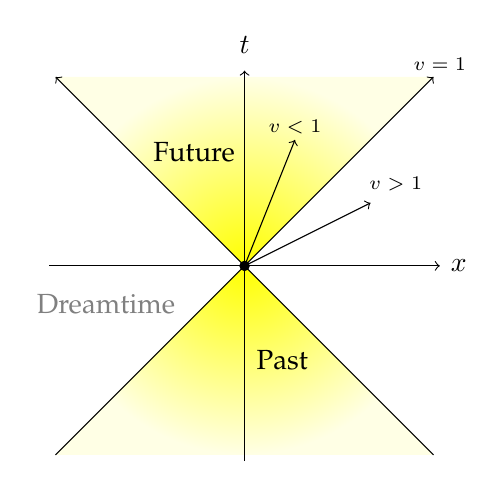
\begin{tikzpicture}
\begin{scope}[scale=0.8]
\shade[inner color=yellow, outer color=yellow!10!white] (-3,-3) -- (0,0) -- (-3,3) -- (3,3) -- (0,0) -- (3,-3) -- (-3,-3);
\draw[->] (-3.1,0) -- (3.1,0);
\draw[->] (0,-3.1) -- (0,3.1);
\draw[color=black,->] (-3,-3)--(3,3);
\draw[color=black,->] (3,-3)--(-3,3);
\draw (0,3.5) node {$t$};
\draw (3.4,0) node{$x$};
\draw[->] (0,0) -- (0.8,2);
\draw[->] (0,0) -- (2,1);
\draw (0.8,2.2) node{\scriptsize $v<1$};
\draw (2.4,1.3) node{\scriptsize $v>1$};
\draw (3.1,3.2) node{\scriptsize$v=1$};
\draw (0.6,-1.5) node{Past};
\draw (-0.8,1.8) node{Future};
\draw[color=gray] (-2.2,-0.6) node{Dreamtime};
\filldraw [black] (0,0) circle (2.1pt);
\end{scope}
\end{tikzpicture}

\column{0.5\textwidth}

{\color{blue} $(\Delta s)^2 = 0$:} Events are {\it lightlike} or 
{\it null separated}, and lie on the surface of a {\it light cone}.\\
\bigskip
{\color{blue} $(\Delta s)^2 < 0$:} Events are {\it timelike separated}, 
lie inside the light cone and constitute the past, present and future 
of an observer at the origin of $\oframe$.\\
\bigskip
{\color{blue} $(\Delta s)^2 > 0$:} Events are {\it spacelike separated}, 
lie outside the light cone, unavailable to an observer at the origin 
of $\oframe$.
\bigskip

\end{columns}
\end{frame}
%%%%%%%%%%%%%%%%%%%%%%%%%%%%%%%%%%%%%%%%%%%%%%%%%%%%%%

%%%%%%%%%%%%%%%%%%%%%%%%%%%%%%%%%%%%%%%%%%%%%%%%%%%%%%
\begin{frame}
\frametitle{Light cones and the interval 2}

Two important points:

\bigskip

\setbeamercolor{lowercol}{fg=black,bg=red!50!white}
\setbeamercolor{uppercol}{fg=black,bg=red!50!white}
\begin{beamerboxesrounded}[upper=uppercol,lower=lowercol,shadow=true]
{All observers agree on what constitutes the past and present, because
$(\Delta s)^2$ is invariant.}
\end{beamerboxesrounded}

\bigskip

\setbeamercolor{lowercol}{fg=black,bg=red!50!white}
\setbeamercolor{uppercol}{fg=black,bg=red!50!white}
\begin{beamerboxesrounded}[upper=uppercol,lower=lowercol,shadow=true]
{Different observers have different light cones and $\therefore$
different pasts, present and futures.}
\end{beamerboxesrounded}

\end{frame}
%%%%%%%%%%%%%%%%%%%%%%%%%%%%%%%%%%%%%%%%%%%%%%%%%%%%%%

%%%%%%%%%%%%%%%%%%%%%%%%%%%%%%%%%%%%%%%%%%%%%%%%%%%%%%
\begin{frame}
\frametitle{Calibrating the axes}

\begin{columns}
\column{0.5\textwidth}

Since $(\Delta s)^2$ is invariant,
\begin{align*}
-t^2 + x^2 & = {\text constant} \\
           & = -\bar{t}^2 + \bar{x}^2
\end{align*}

The dashed curves in the figure show $-t^2 + x^2 = -1$ (red, locus of
spacelike constant interval events) and $-t^2 + x^2 = 1$ (green, locus 
of timelike constant interval events).  These {\it\color{red} invariant hyperbolae}
are asymptotic with a light path through the origin.

\column{0.5\textwidth}
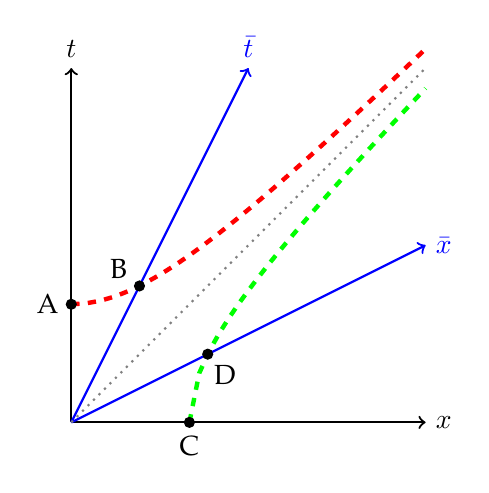
\begin{tikzpicture}[scale=1.5]
% O'S AXES
\draw [->,thick] (0,0) -- (0,3) node [above] {$t$};
\draw [->,thick] (0,0) -- (3,0) node [right] {$x$};
% OBAR'S axis
\draw [->,thick,blue] (0,0) -- (1.5,3) node [above] {$\bar{t}$};
\draw [->,thick,blue] (0,0) -- (3,1.5) node [right] {$\bar{x}$};
% INVARIANT HYPERBOLAE
\draw [red,ultra thick,dashed,domain=0:3] plot (\x, {sqrt(1 + \x*\x) });
\draw [green,ultra thick,dashed,domain=1:3] plot (\x, {sqrt(\x*\x - 1) });
% EVENTS
\filldraw [black] (0,1) circle (1.2pt);
\node at (-0.2,1) {A};
\filldraw [black] (1,0) circle (1.2pt);
\node at (1,-0.2) {C};
\filldraw [black] (0.5774,1.155) circle (1.2pt);
\node at (0.4,1.3) {B};
\filldraw [black] (1.155,0.5774) circle (1.2pt);
\node at (1.3,0.4) {D};
% PHOTON PATH
\draw [-,dotted,thick,gray] (0,0) -- (3,3);
\end{tikzpicture}

\end{columns}
\end{frame}
%%%%%%%%%%%%%%%%%%%%%%%%%%%%%%%%%%%%%%%%%%%%%%%%%%%%%%

%%%%%%%%%%%%%%%%%%%%%%%%%%%%%%%%%%%%%%%%%%%%%%%%%%%%%%
\begin{frame}[fragile]{Homework}
\begin{columns}
\column{\textwidth}
\setbeamercolor{uppercol}{fg=white,bg=red!54!black}
\setbeamercolor{lowercol}{fg=black,bg=red!10}
\begin{beamerboxesrounded}[upper=uppercol,lower=lowercol,shadow=true]{Homework 2}

1. Work carefully and thoroughly through each step of slides 19 -- 28 of these
lecture slides, i.e. the first--principles proof of interval invariance.\\

\bigskip

2. Do problems 1 -- 4 inclusive on Tutorial Sheet 1
{\tiny
\begin{verbatim} 
(http://www.phys.unsw.edu.au/~jkw/phys3550/PHYS3550_tuts1-5_withsolutions.pdf).
\end{verbatim}
}
Make sure you attempt them first before you look at the solutions supplied.

\end{beamerboxesrounded}
\end{columns}
\end{frame}
%%%%%%%%%%%%%%%%%%%%%%%%%%%%%%%%%%%%%%%%%%%%%%%%%%%%%%


\end{document}
